% Fig. 4.7 -- 三條 t 密度曲線 (自由度 1、3、10) 與標準常態密度曲線疊在同一組
%   座標軸上。
% 書稿來源: mathstatch4.tex 第 4168 至 4200 行的 tikzpicture (pgfplots 的 axis
%   環境，width=.8\textwidth、height=.45\textwidth)。
%
% 密度: f(t) = K_nu * (1 + t^2/nu)^{-(nu+1)/2}，
%   K_nu = Gamma((nu+1)/2) / ( sqrt(nu pi) Gamma(nu/2) )。三個常數由 lgamma 另行
%   算出並寫死在下面: K_1 = 0.3183099、K_3 = 0.3675526、K_10 = 0.3891084;
%   標準常態則是 0.3989423 e^{-t^2/2}。冪次一律改寫為 exp(-((nu+1)/2) ln(1+t^2/nu))，
%   指數項為非正數，pgfmath 不會溢位。
%
% 對書稿的三處調整:
%   1. 第四條曲線: 書稿畫的是 student(x,100)，也就是自由度 100 的 t 密度，圖例
%      卻標為 N(0,1)。本檔改畫真正的標準常態密度，與圖例、與正文所談的對照
%      對象一致。兩者在本圖的尺度下相差不到 0.00127 個密度單位，換算為
%      0.0136cm，不到一個線寬的一半，肉眼無從分辨。**此點待作者裁定**，
%      候選稿的 fig-pending 註解已列為待決事項，若作者裁定照書稿保留 t(100)，
%      把下面 normal 那一條改回 0.3979462*exp(-50.5*ln(1+\x*\x/100)) 即可。
%   2. 線型: 書稿為實線、dotted、dashed、粗實線。本檔依 CH2_FIGURE_SPECS 1.9 節
%      以線型加圖例兩重識別，一律 journalink: 標準常態是比較的基準，取 1.0pt
%      實線; t(10) 取 on 4pt off 2pt、t(3) 取 on 1pt off 2pt、t(1) 取點劃線
%      on 4pt off 1.5pt on 0.8pt off 1.5pt。同節只固定三種線型，四條曲線需要
%      第四種，點劃線是與既有三種距離最遠的一種。
%   3. 書稿設了 ylabel 為 $f_T(t)$，但同時設 axis y line=none，實際上不會顯示，
%      本檔一併不畫縱軸與縱軸名。
%
% 標示: 四條曲線在峰頂附近彼此相距不到 0.08 個密度單位、在尾部更擠在一起，
%   曲線末端無法直接掛標示，故依 1.9 節的備案在右上角放圖例，短線段長 0.5cm。
%   圖例最低一列在 y=0.299，該處以右各曲線的高度都不到 0.034，留白充足。
%
% 座標: x 由 -6.2 到 6.4、刻度為 -6 至 6 的十三個整數 (照書稿)，y 由 0 到 0.45
%   (照書稿)。x=0.68cm、y=10.7cm，繪圖範圍 8.57cm 寬、4.82cm 高，寬高比 0.562，
%   與書稿的 .8:.45 = 0.5625 相同。刻度標籤相鄰間距 0.68cm，標籤本身寬約
%   0.45cm，留白 0.23cm。
%
% 產製:
%   pdflatex student-t-density-family.tex
%   pdftocairo -svg student-t-density-family.pdf \
%     ../../images/teaching-topics/student-t-density-family.svg

\documentclass[tikz,border=2pt]{standalone}
\usepackage{amsmath}
\usepackage{amssymb}
\usepackage{xcolor}
\usetikzlibrary{arrows.meta}

%% 圖內沒有下標，最小字即 10pt 的內文級。
\DeclareMathSizes{10}{10}{9}{9}

\definecolor{journalink}{HTML}{1F1C18}
\definecolor{journalmuted}{HTML}{8A7F72}
\definecolor{journalaccent}{HTML}{9C2D2D}

\begin{document}
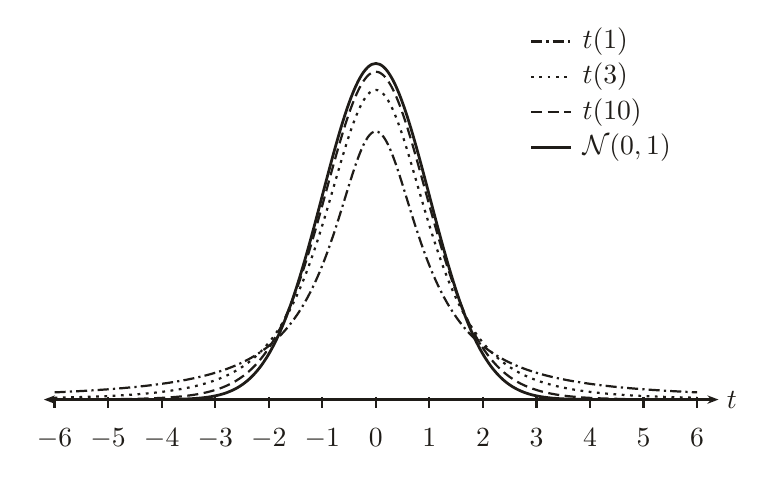
\begin{tikzpicture}[
  x=0.68cm,
  y=10.7cm,
  every node/.style={font=\normalsize, journalink},
  axis/.style={journalink, line width=0.8pt,
               {Stealth[length=4pt]}-{Stealth[length=4pt]}},
  tick/.style={journalink, line width=0.8pt},
  curvenormal/.style={journalink, line width=1.0pt},
  curveten/.style={journalink, line width=0.8pt,
                   dash pattern=on 4pt off 2pt},
  curvethree/.style={journalink, line width=0.8pt,
                     dash pattern=on 1pt off 2pt},
  curveone/.style={journalink, line width=0.8pt,
                   dash pattern=on 4pt off 1.5pt on 0.8pt off 1.5pt}
]
  %% ---- 四條密度曲線 ------------------------------------------------------
  %% t(1): K = 0.3183099
  \draw[curveone] plot[domain=-6:6, samples=161, smooth]
    (\x,{0.3183099*exp(-1*ln(1+\x*\x))});

  %% t(3): K = 0.3675526
  \draw[curvethree] plot[domain=-6:6, samples=161, smooth]
    (\x,{0.3675526*exp(-2*ln(1+\x*\x/3))});

  %% t(10): K = 0.3891084
  \draw[curveten] plot[domain=-6:6, samples=161, smooth]
    (\x,{0.3891084*exp(-5.5*ln(1+\x*\x/10))});

  %% 標準常態
  \draw[curvenormal] plot[domain=-6:6, samples=161, smooth]
    (\x,{0.3989423*exp(-\x*\x/2)});

  %% ---- x 軸 --------------------------------------------------------------
  \draw[axis] (-6.2,0) -- (6.4,0);
  \node[anchor=west, inner sep=2.8pt] at (6.4,0) {$t$};

  \foreach \p in {-6,-5,-4,-3,-2,-1,0,1,2,3,4,5,6}
    \draw[tick] ([yshift=0.035cm]\p,0) -- ([yshift=-0.106cm]\p,0);
  \foreach \p in {-6,-5,-4,-3,-2,-1,0,1,2,3,4,5,6}
    \node[anchor=north] at ([yshift=-0.25cm]\p,0) {$\p$};

  %% ---- 圖例，右上角 ------------------------------------------------------
  %% 短線段由 x=2.90 到 x=3.64 (0.5cm)，文字起於 x=3.85。
  \draw[curveone] (2.90,0.425) -- (3.64,0.425);
  \node[anchor=west, inner sep=0pt] at (3.85,0.425) {$t(1)$};

  \draw[curvethree] (2.90,0.383) -- (3.64,0.383);
  \node[anchor=west, inner sep=0pt] at (3.85,0.383) {$t(3)$};

  \draw[curveten] (2.90,0.341) -- (3.64,0.341);
  \node[anchor=west, inner sep=0pt] at (3.85,0.341) {$t(10)$};

  \draw[curvenormal] (2.90,0.299) -- (3.64,0.299);
  \node[anchor=west, inner sep=0pt] at (3.85,0.299) {$\mathcal{N}(0,1)$};
\end{tikzpicture}
\end{document}
